\documentclass{article}
\usepackage{indentfirst}
\usepackage{blindtext}
\usepackage{graphicx}
\usepackage{wrapfig}
% \usepackage{subfig}
\usepackage{subcaption}

\title{Skills Assessment}
\author{Nathan Givens}
\date{November 8, 2019}

\setlength{\parindent}{4ex}

\begin{document}

  \maketitle

  \section{UART Bus Decoding}

  \subsection{Required Equipment}

  UART bus decoding is a method of capturing communications over a UART bus and
  decoding the information sent between devices. Equipment often decodes the
  information into hexadecimal, but the equipment available in the labs can
  display the information in binary and ASCII as well. The procedure described
  in this document should apply to any of the oscilloscopes available in the
  senior design labs but was prepared using a Keysight MS0-X 3014T so there may
  be some subtle differences between models.

  \begin{figure}[h]
    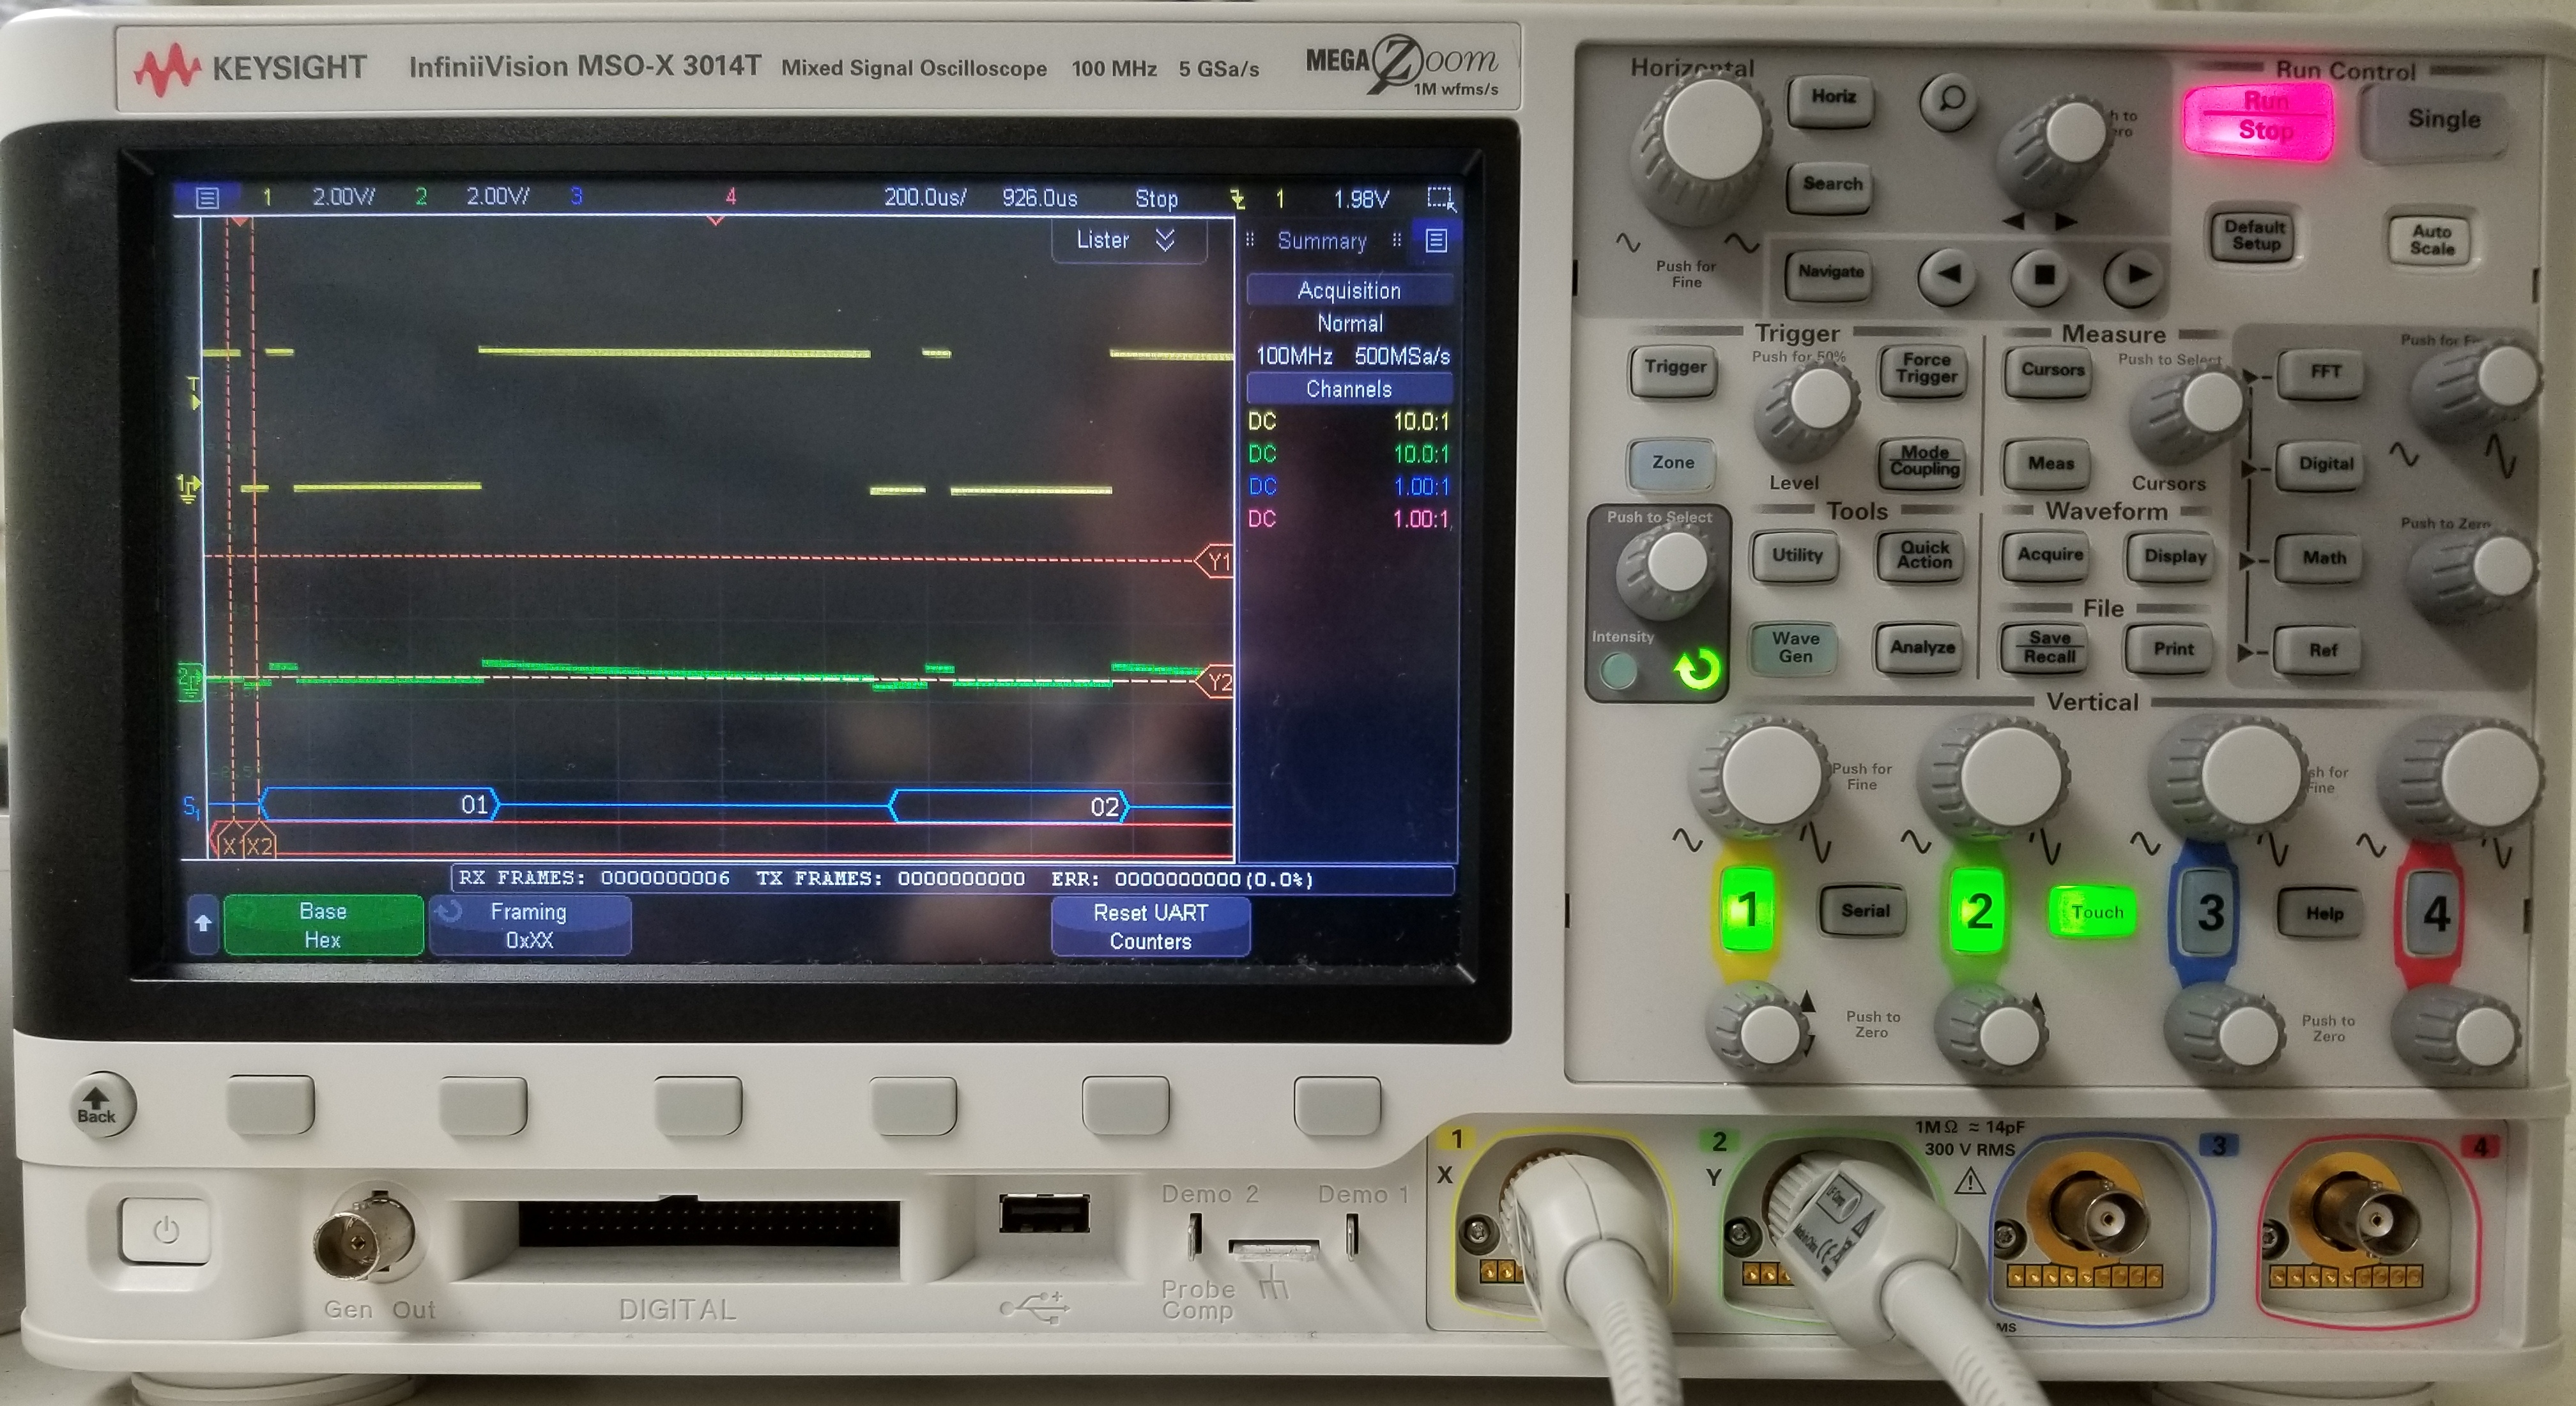
\includegraphics[width=\textwidth]{images/uart/full_scope.jpg}
    \caption{An oscilloscope properly decoding data from a UART bus}
  \end{figure}

  \subsection{Setup}

  Firstly, the oscilloscope must be turned on and the proper number of probes
  must be connected. For UART, two cables are needed to test two way
  asynchronous communications. If only one signal needs to be decoded, then only
  one cable needs to be connected to the oscilloscope. However, having more
  cables connected to the oscilloscope won't hurt anything, it may just clutter up
  available work space.

  \begin{wrapfigure}{l}{44ex}
    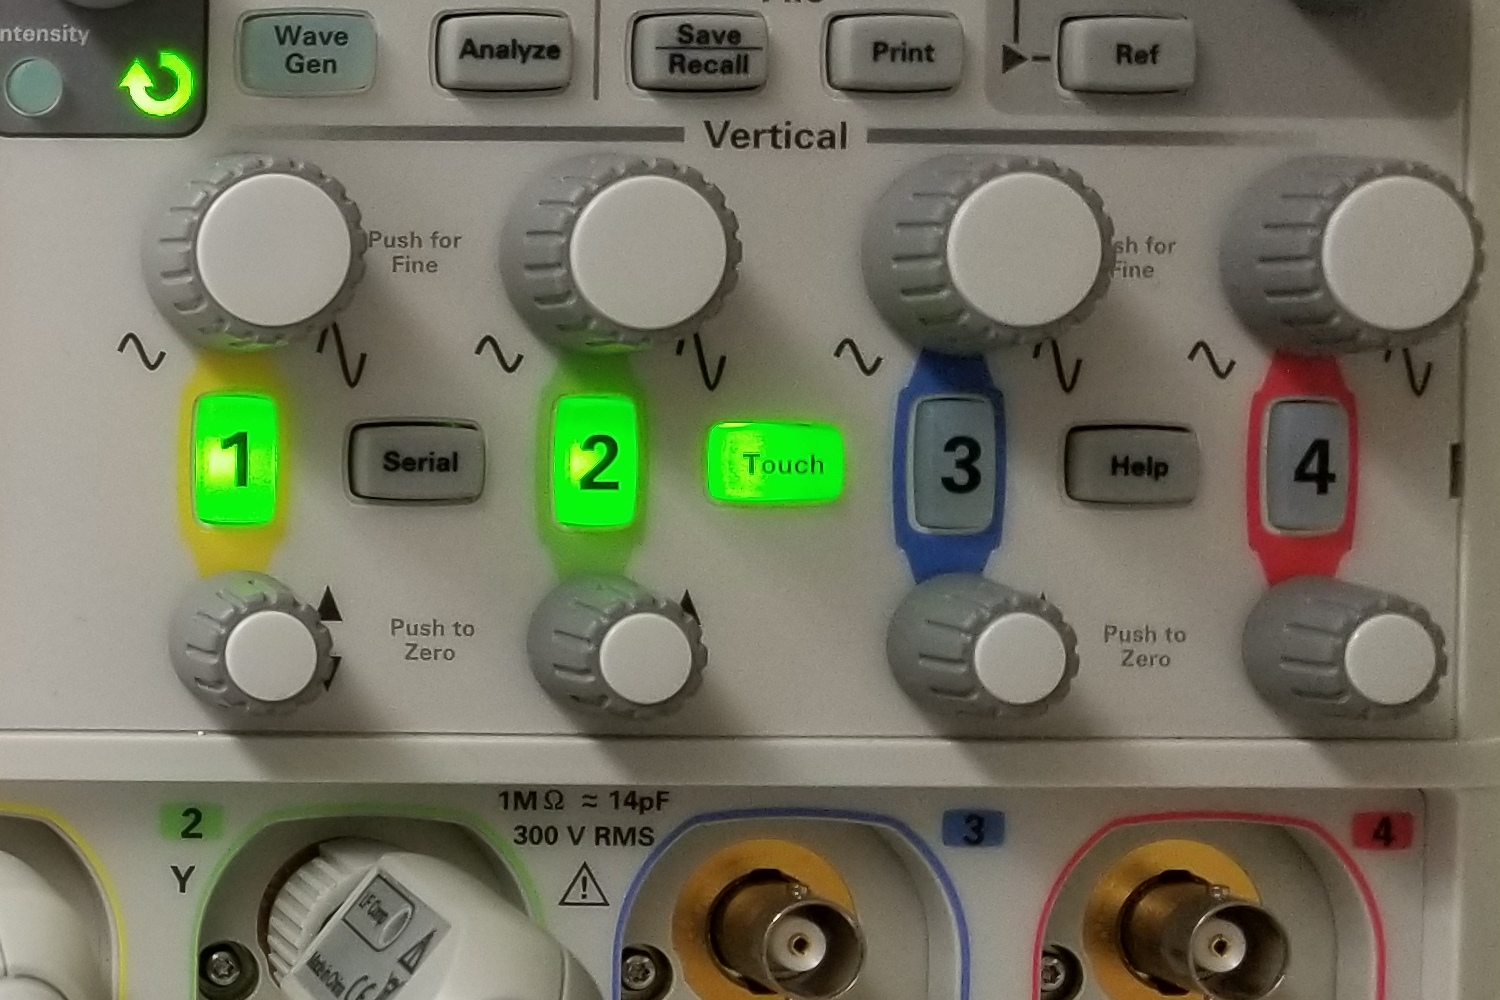
\includegraphics[width=44ex]{images/uart/serial_button_scope.jpg}
    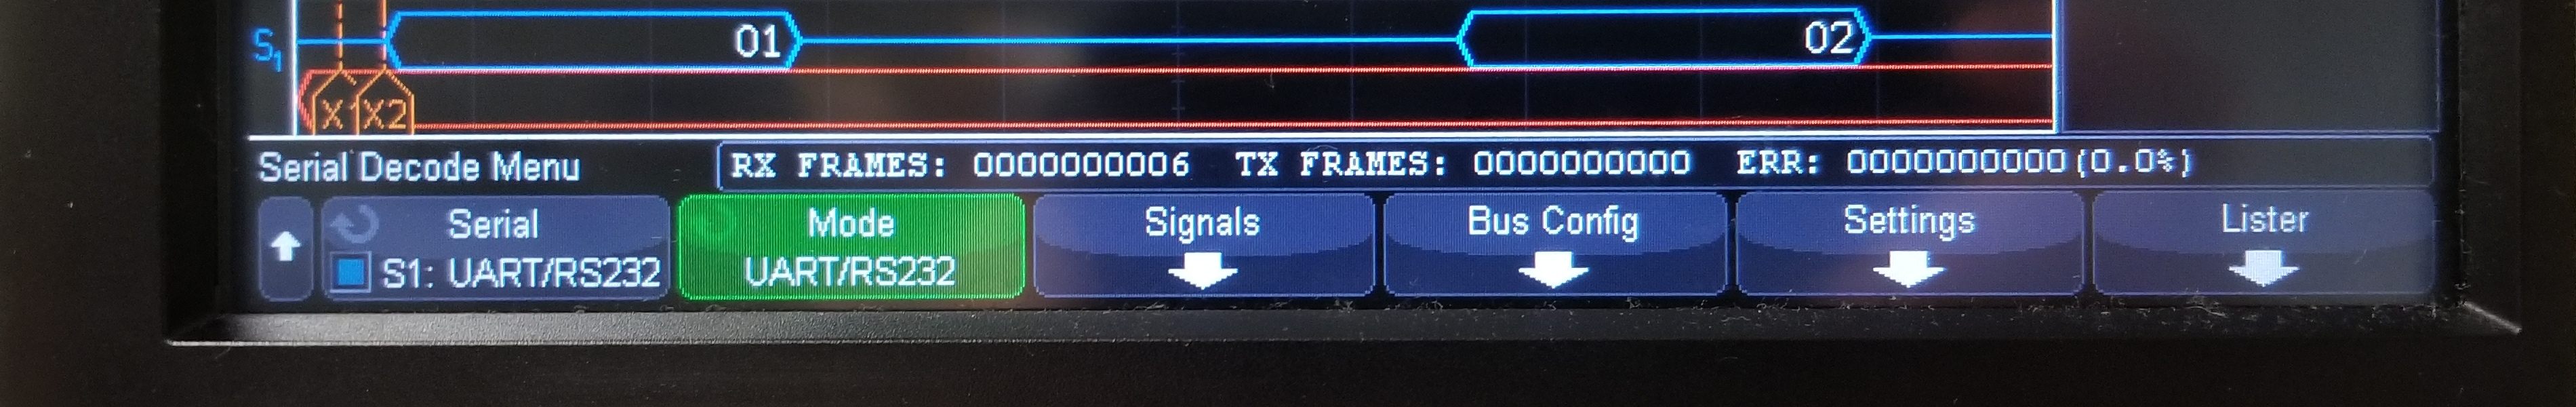
\includegraphics[width=44ex]{images/uart/serial_decode_scope.jpg}
    \caption{Serial button located between buttons 1 and 2. Serial Decode Menu,
      shown with UART/RS232 selected.}
  \end{wrapfigure}

  The oscilloscopes have a Serial button located between buttons 1 and 2.
  Pressing this button opens the serial protocol decoding menu at the bottom of
  the display. The menu changes according to the selected protocol. This menu
  holds all of the settings associated with serial bus deocing. This
  document will discuss some of the various settings that are available, and
  walk through an example of configuring the scope to properly decode a UART bus
  communication.

  \begin{wrapfigure}[18]{r}{25ex}
    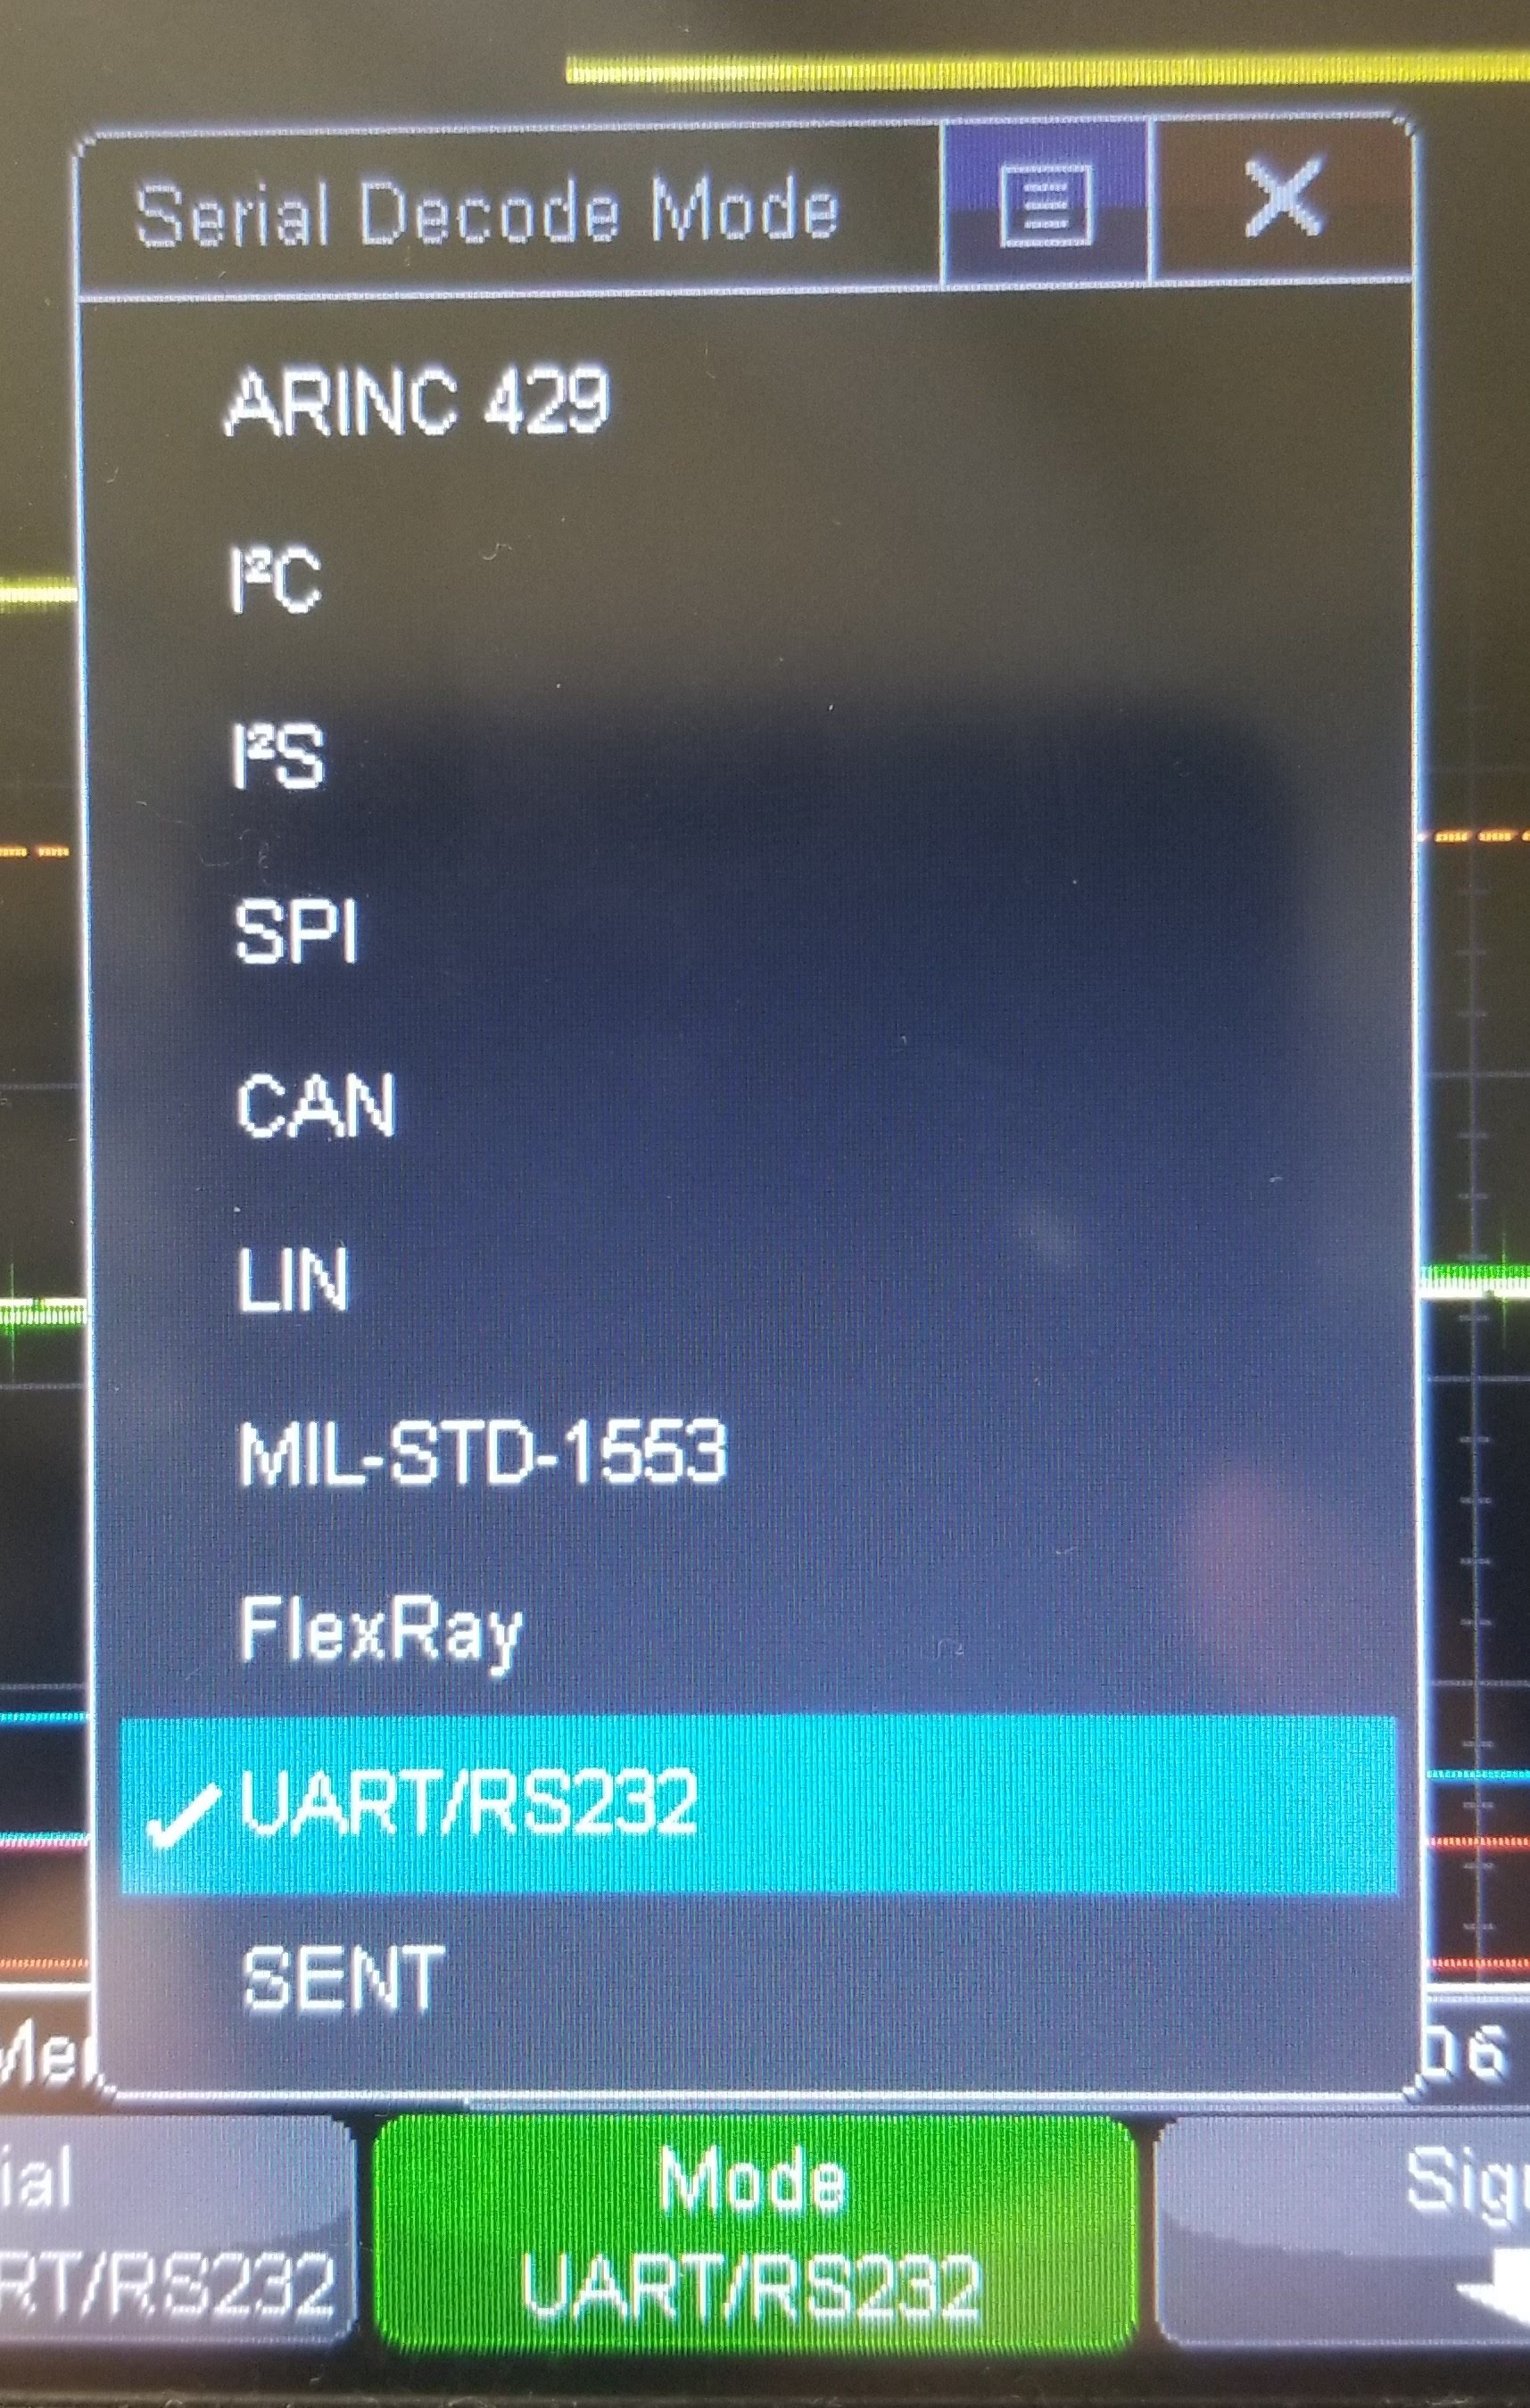
\includegraphics[width=25ex]{images/uart/mode_menu.jpg}
    \caption{Mode selection menu on oscilloscope}
    \label{fig:uart_mode_menu}
  \end{wrapfigure}

  Inside the serial menu, the mode needs to be set to reflect the expected
  communication. Conveniently, the mode button allows this configuration to be
  made. Pressing the mode button reveals a list of communication protocols that
  the oscilloscope can decode. Because this section describes UART communication
  decoding, UART/RS232 is selected from the list. Other sections of this
  document discuss some of the other protocols listed here. After UART/RS232 is
  selected, all submenus update to display settings
  specific to decoding UART.

  % Signals submenu
  The signals submenu gives the ability to specify which input is associated
  with which signal. In the case of UART, the availbalbe signals are Rx and Tx.
  In the example, channel 1 is set to Rx and receives the signals that are
  leaving through the devices Tx connection. The channel could be connected to
  either Rx or Tx from the device, but sticking with convention should help
  prevent confusion while debugging. The thresholds for signals can also be
  adjusted here in case different voltages are being used. The threshold shown
  in Figure~\ref{fig:uart_signals_menu} for Rx was set to just above the
  threshold for logic high in the device meant to receive the signals. The Tx
  signal was not set because, for this example, no Tx signal connected. Now that
  the signals are properly correlated to the correct channels, the bus settings
  can be configured so signals can be properly decoded.

  \clearpage

  \begin{figure}[h]
    \centering
    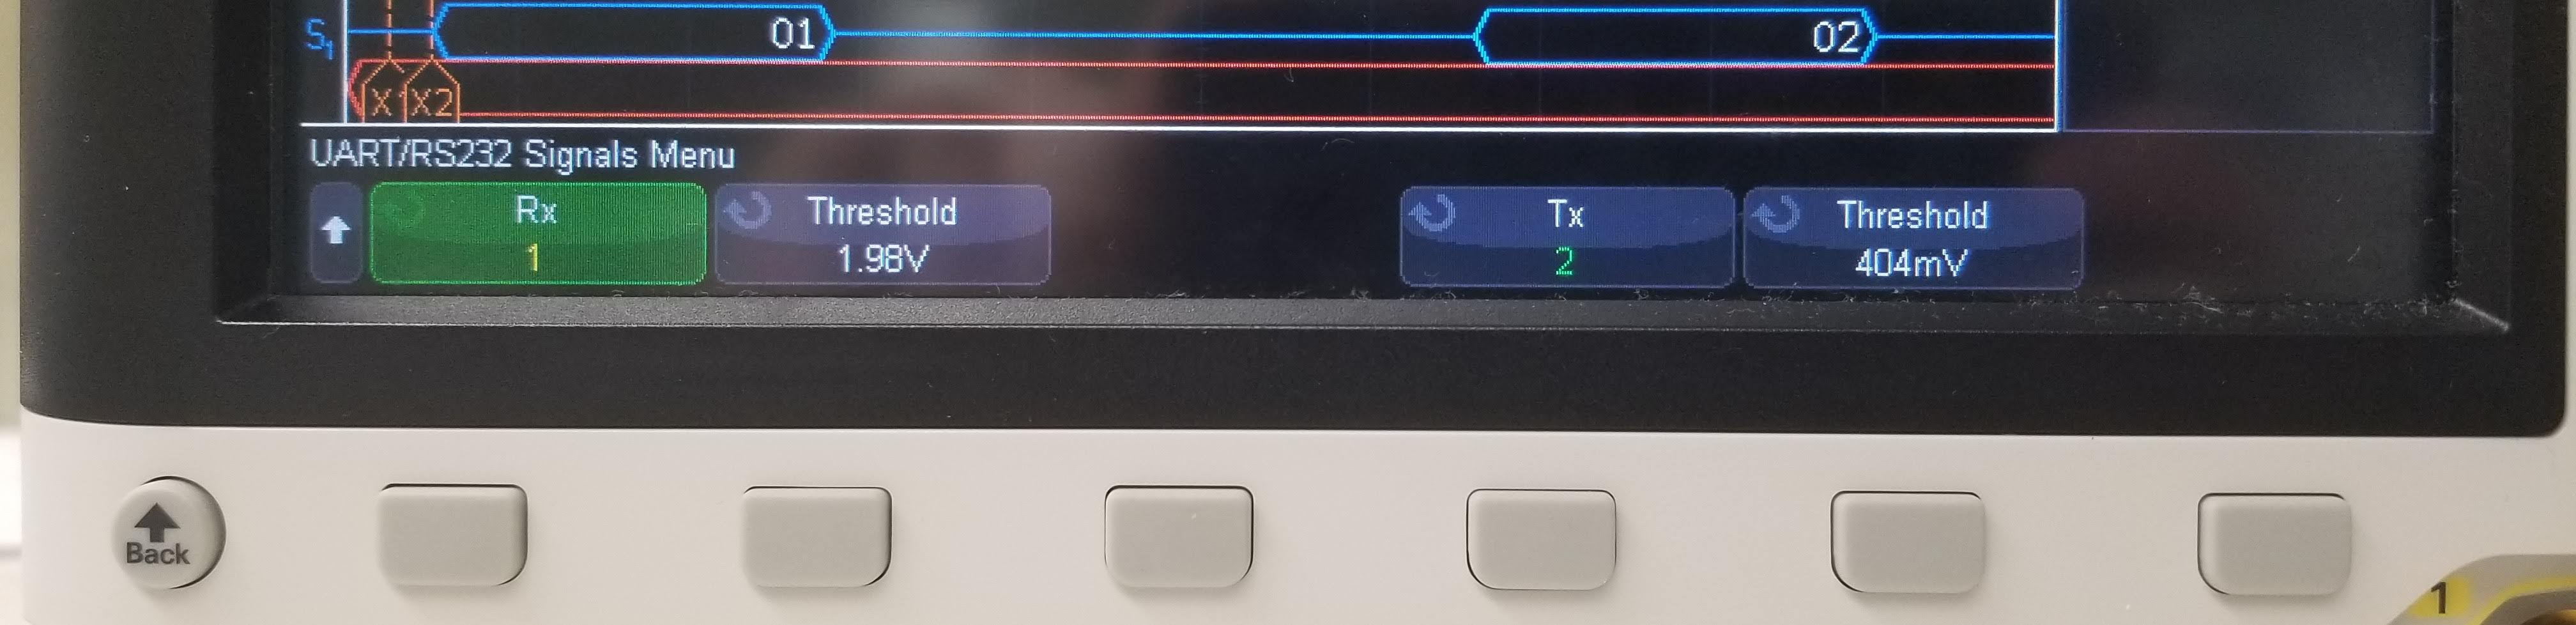
\includegraphics[width=0.9\textwidth]{images/uart/signals_menu.jpg}
    \caption{Signals submenu showing channel 1 as Rx with a threshold of 1.98V}
    \label{fig:uart_signals_menu}
  \end{figure}

  % Bus Configuration
  The configurations for UART communication are located in the Bus Config Menu.
  The number of bits, parity (if any), baud rate, idle polarity, and bit order
  can be adjusted here to match the expected transmission settings. The baud
  rate is adjusted from within a submenu where a value can be entered directly.
  This example uses eight bit transmissions without a parity bit, an idle line
  will remain at logic high, and the bits are transmitted Least Significant
  Bit first. This example was recorded at 19,200 baud.

  \begin{figure}[h]
    \centering
    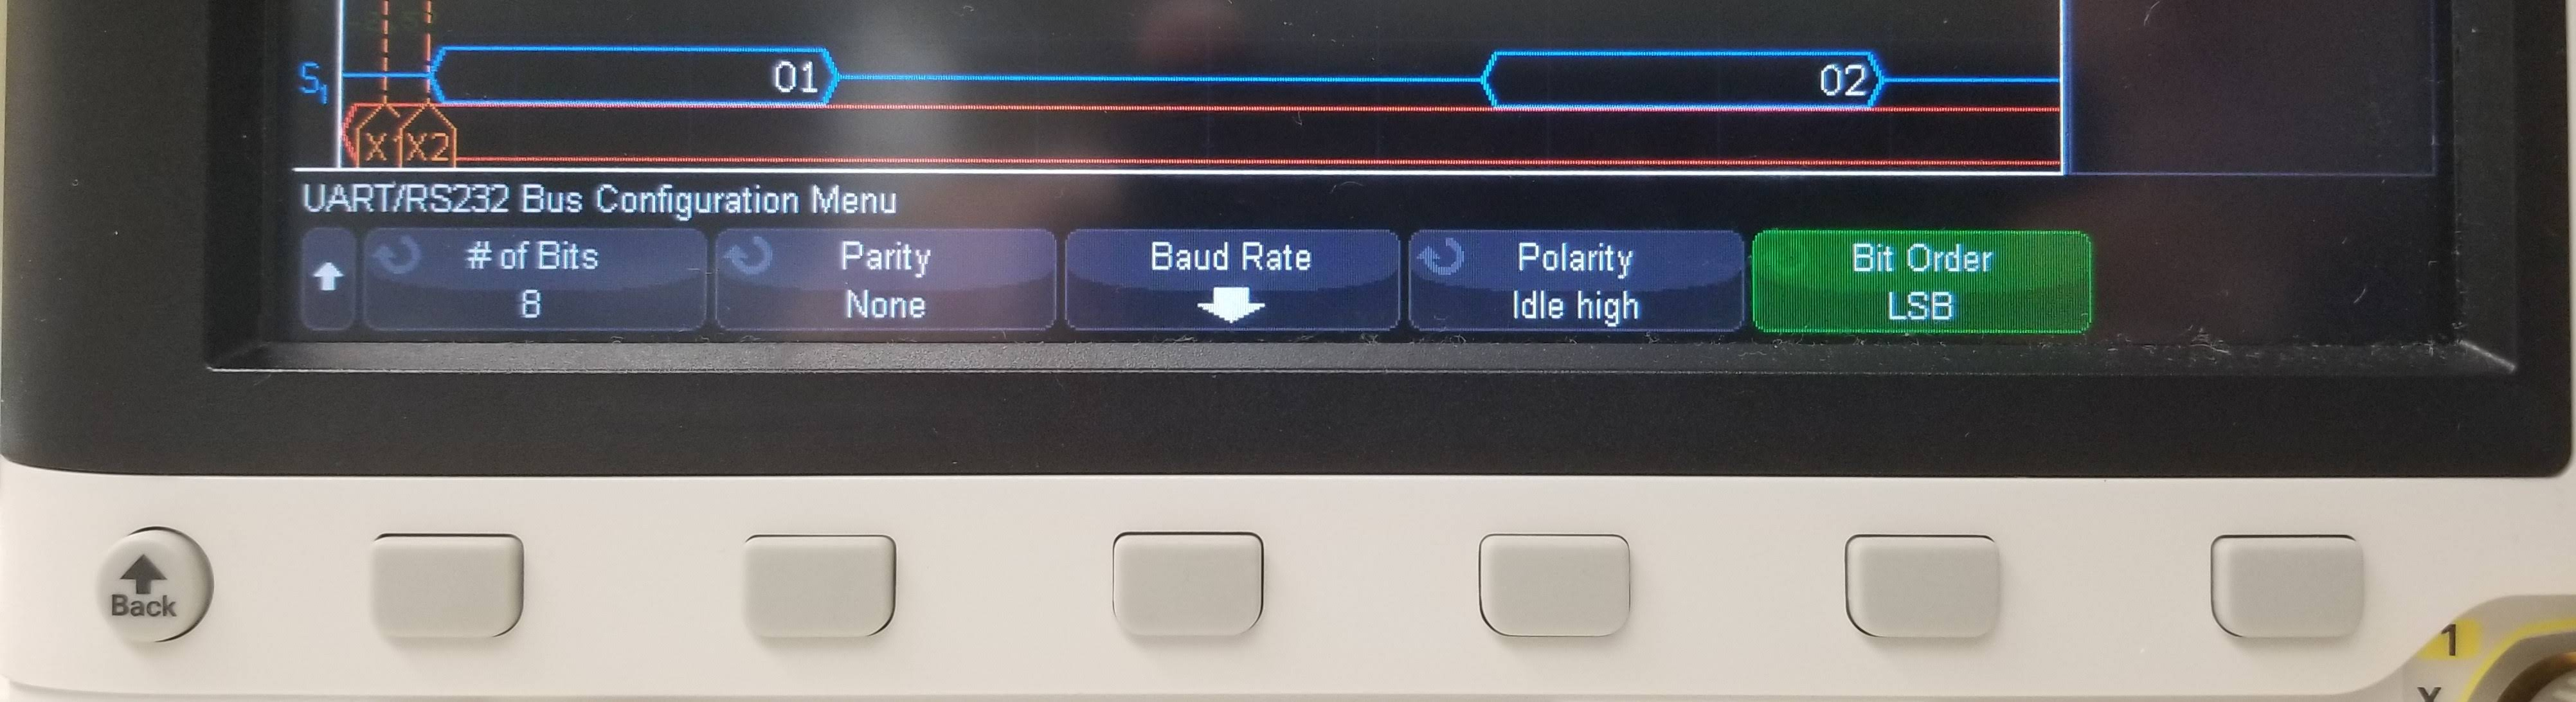
\includegraphics[width=0.9\textwidth]{images/uart/bus_config.jpg}
    \caption{UART/RS232 Bus Configuration Menu}
  \end{figure}

  % Settings
  Inside the settings menu, the base number for displayed values can be
  selected. The example is currently set to hex, so all numbers displayed are
  hexadecimal. The framing size for displayed information can also be adjusted.
  Currently, the framing size is set to two, so the information is broken into
  two hexadecimal numbers per frame. This was chosen in the example because it
  matches the size of data frames that are sent. The oscilloscope will also keep
  a running total of frames it has received, and the last button in this submenu
  can reset that running total. This can be useful to ensure the proper number
  of data frames when trying to decode long message sequences.

  % Lister Menu
  The oscilloscope has a lister functionality. The lister will display the list
  of data the oscilloscope has received and decoded as well as any errors
  detected with a data frame. The lister can be displayed from within this menu.
  This document only shows the navigation through the softkeys; however, if
  touch functionality is availbable, a button on the touchscreen near the top
  righthand side of the display can also open the lister display.  Inside the
  settings menu, the base number for displayed values can be selected. The
  example is currently set to hex, so all numbers displayed are hexadecimal. The
  framing size for displayed information can also be adjusted.  Currently, the
  framing size is set to two, so the information is broken into two hexadecimal
  numbers per frame. This was chosen in the example because it matches the size
  of data frames that are sent. The oscilloscope will also keep a running total
  of frames it has received, and the last button in this submenu can reset that
  running total. This can be useful to count data frames when working with long
  communications.

  \begin{figure}[ht]
    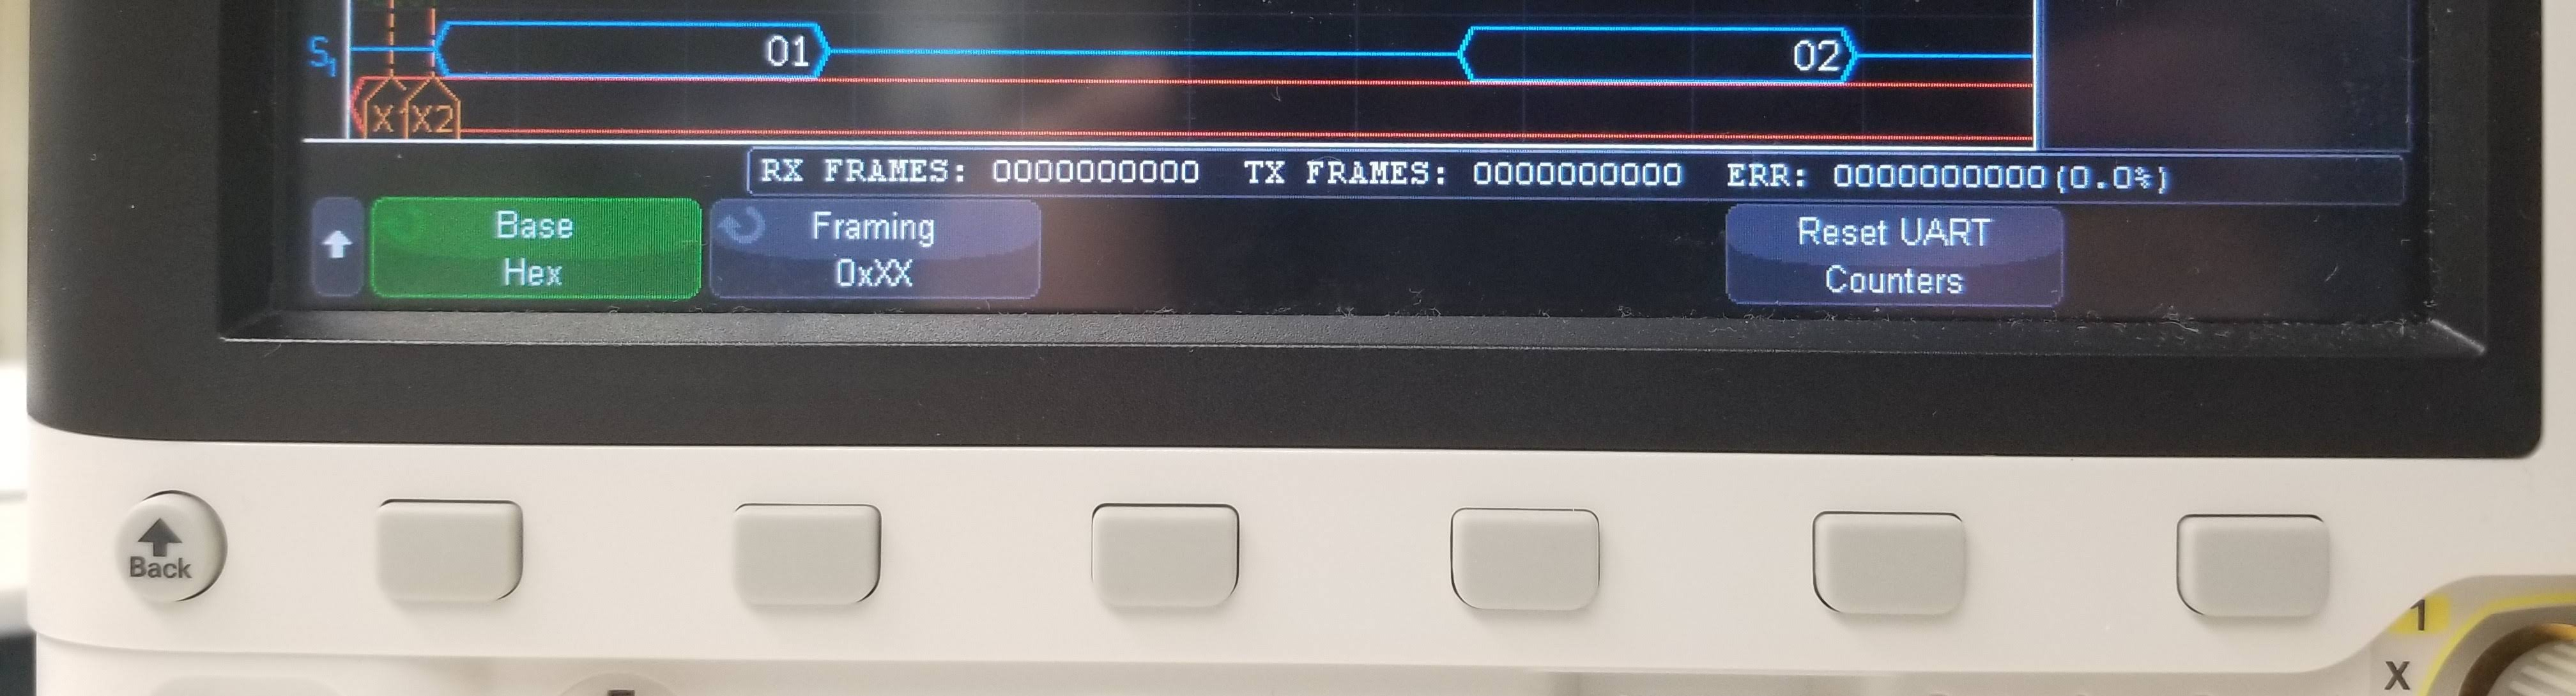
\includegraphics[width=\textwidth]{images/uart/uart_settings.jpg}
    \caption{Settings submenu for UART configuration}
  \end{figure}

  \subsection{Results}

  \begin{figure}[ht]
    \subfloat[]{
      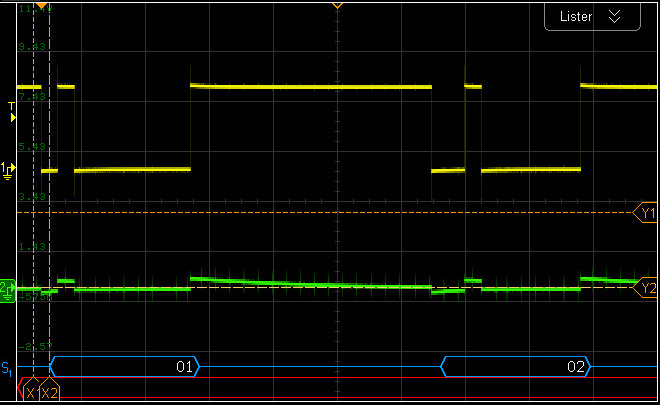
\includegraphics[width=0.5\textwidth]{images/uart/uart_bus.jpg}
    }
    \subfloat[]{
      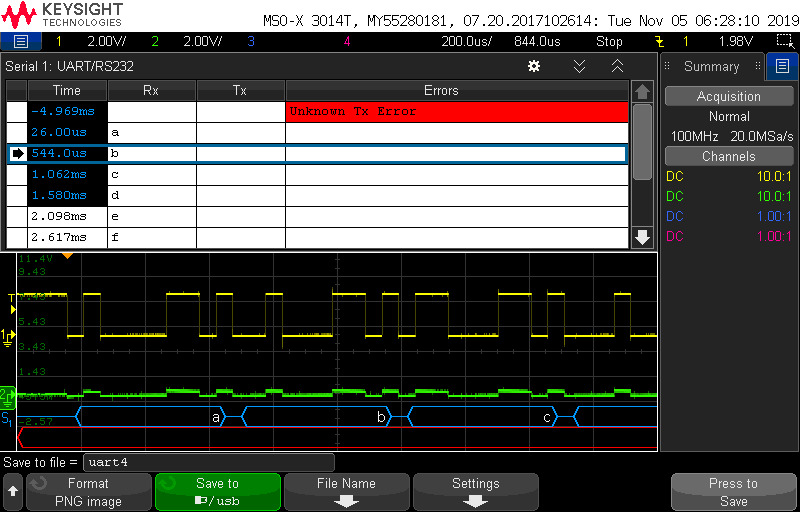
\includegraphics[width=0.5\textwidth]{images/uart/lister.jpg}
    }
    \caption{Decoded UART signals with and without lister menu.}
    \label{fig:uart_bus}
  \end{figure}

  When the oscilloscope detects a data frame, it will decode the signals it
  receives and display those values at the bottom of the screen as shown in
  Figure~\ref{fig:uart_bus}. The blue signals represent the Rx signals that were
  decoded. If a Tx signal had been measured, its values would be displayed in
  the red signals at the bottom of the screen. Figure~\ref{fig:uart_bus}a shows
  0x01 and 0x02, the expected data, were received. In
  Figure~\ref{fig:uart_bus}b, the lister menu can be seen displaying a list of
  the decoded signals that were received in the last transmission.

  \section{SPI Bus Decoding}

  \subsection{Required Equipment}

  The oscilloscopes available in the labs can also be used to decode SPI Bus
  communications. The configuration process is similar to that used for UART
  decoding, so it will be covered in slightly less detail in this section.

  \subsection{Setup}

  The setup for SPI bus decoding begins by selecting SPI from the mode menu that
  was discussed in the previous section. Selecting SPI updates all the submenus
  with settings for SPI decoding allowing proper configuration.

  \begin{figure}[h]
    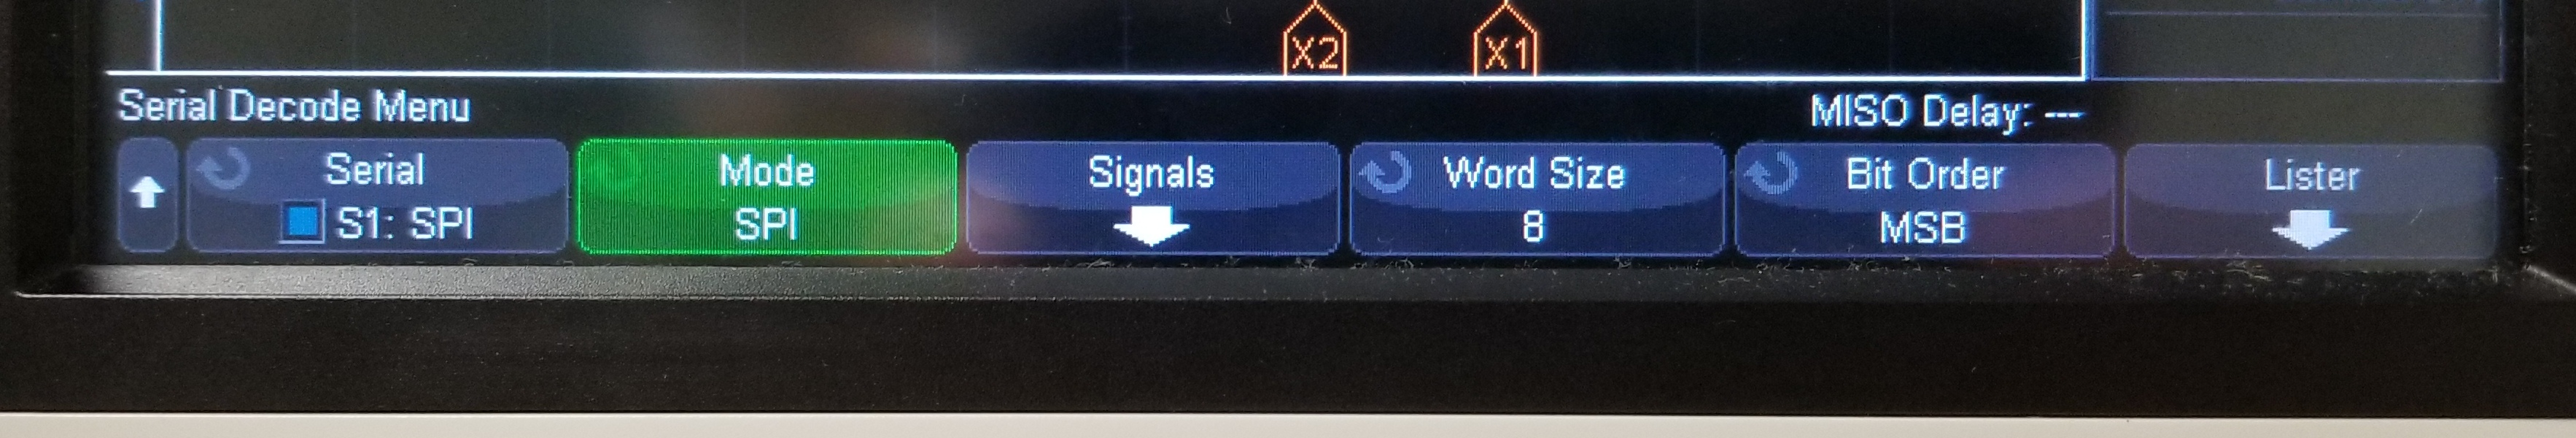
\includegraphics[width=\textwidth]{images/spi/spi_serial_menu.jpg}
    \caption{SPI Serial Decode Menu}
  \end{figure}

  % Signals
  The Signals submenu works identically to the previously described Signals
  submenu. The only difference is that now the signals listed are the standard
  signals used in SPI communication (CLK, CS, MOSI, and MISO). When Setting the
  MISO signal, there is an extra parameter to allow for a delay from the
  selected device.

  \begin{figure}[h]
    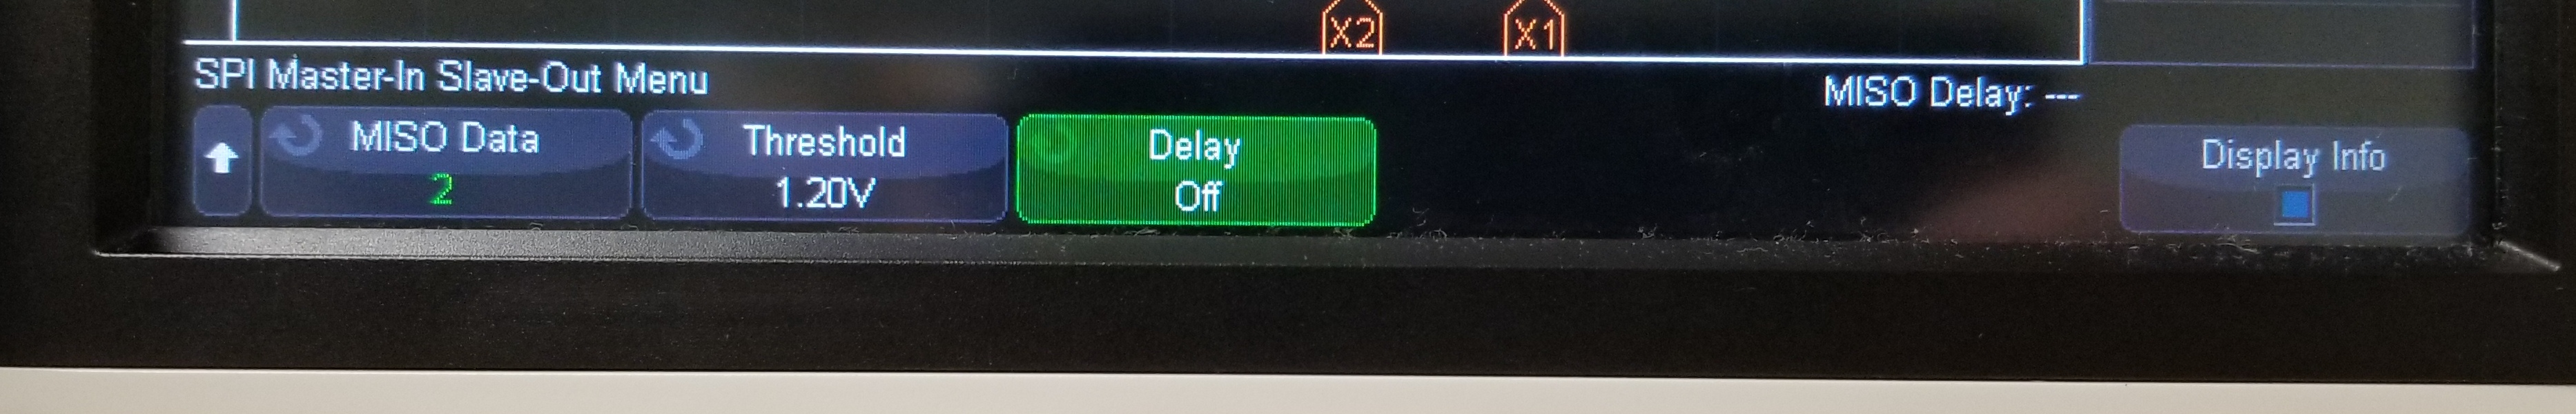
\includegraphics[width=\textwidth]{images/spi/spi_slave_delay.jpg}
    \caption{SPI MISO signal delay menu}
  \end{figure}

  % Word Size
  The word size should now be adjusted to set the meaningful data frame size.
  Because SPI has a clock associated with it, a transmission can continue
  without breaking in between data frames, so the oscilloscope needs to be told
  where data boundaries are expected.
  % Bit Order
  Similarly to any other serial bus protocol, the endianness of the transmission
  must be specified. In the examples, the signals will be sent Most Significant
  Bit First.
  %Lister
  The lister is also available to the user when decoding SPI bus signals.

  \subsection{Results}

  % TODO get images for this
  % TODO Write program for esp32 to send fake data
  The oscilloscope should now show the data that was detected in the lines. The
  values are displayed in hexadecimal at the bottom on the screen, or, as
  mentioned before, the lister menu will also display the detected information.
  Figure~\ref{fig:spi_bus} shows a message recieved with values 61, 62, and 63.
  These are the hexadecimal values that represent the letters a, b, and c, the
  information that was sent over the bus.

  \begin{figure}[ht]
    \begin{subfigure}[b]{0.5\textwidth}
      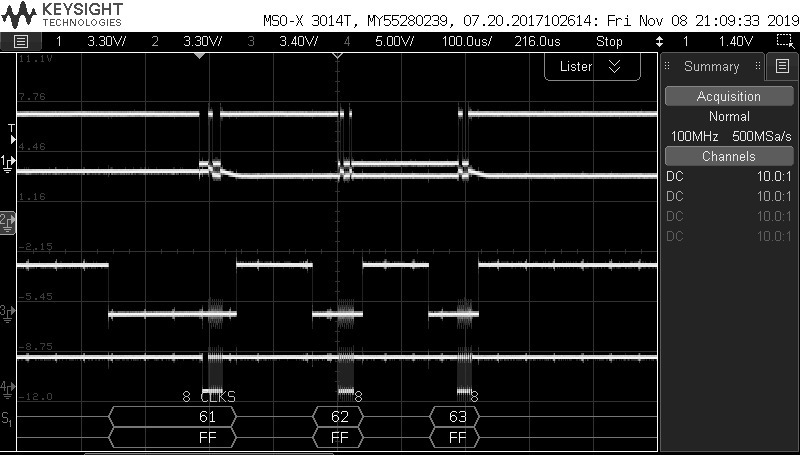
\includegraphics[width=\linewidth]{images/spi/spi_bus.jpg}
      \caption{}
    \end{subfigure}
    \begin{subfigure}[b]{0.5\textwidth}
      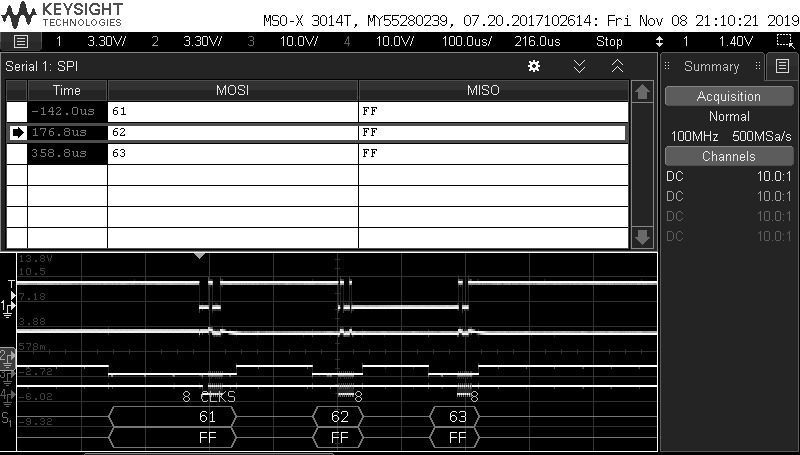
\includegraphics[width=\linewidth]{images/spi/spi_bus_lister.jpg}
      \caption{}
    \end{subfigure}
    \caption{decoded SPI data}
    \label{fig:spi_bus}
  \end{figure}

  \section{I\textsuperscript{2}C Bus Decoding}

  \subsection{Required Equipment}

  Oscilloscopes, being the useful tools that they are, can also decode
  I\textsuperscript{2}C
  serial buses. They provide some extra insight about the information decoded
  from an I\textsuperscript{2}C bus by highlighting the data to make it easier to quickly read and
  understand. Address bytes are colored depending on it being a read or write
  command, and the data that is transferred in a communication cycle is
  displayed in white text. The oscilloscope also displays a 'R' or an 'W' with
  command bytes to signify Read or Write commands. An 'a' or '~a' for ACK or
  NACK will be displayed for each byte transmitted.

  \subsection{Setup}

  To begin, as always, the type of serial bus must be specified. As before, the
  channels must be assigned to the corresponding signals so they may be decoded
  properly. In this example, channel two is SCL and channel one is SDA.
  I\textsuperscript{2}C
  devices use designated addresses. The addresses are typically seven bits, as
  it is with this example, but could also be eight bits long. Address length
  must therefore be specified.

  \subsection{Results}

  The oscilloscope displays the decoded message at the bottom of the screen and
  in the lister menu if desired. Figure~\ref{fig:i2c_decode} shows a complete
  communication sequence between a master and a slave device. We can see the
  master send a write byte to the slave's address and the data sent afterwards
  is a byte to tell the slave to return information from one its registers. The
  next byte sent from the master device signals that it wishes to read the
  value, and the following data is sent from the slave.

  \begin{figure}[ht]
    \begin{subfigure}[b]{.5\textwidth}
      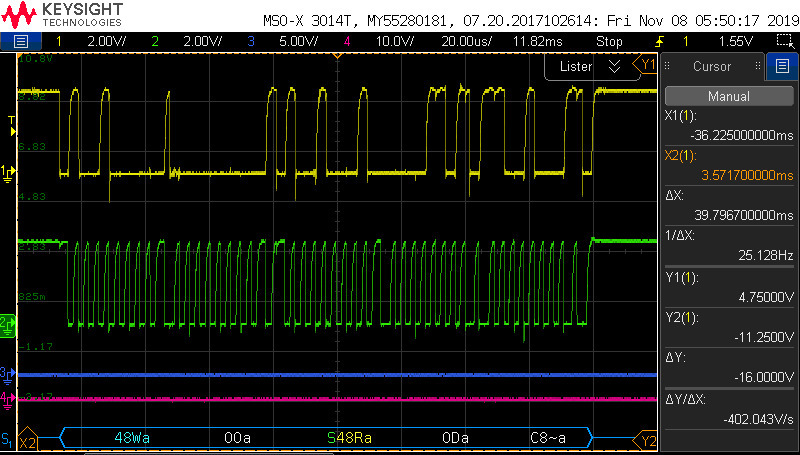
\includegraphics[width=\linewidth]{images/i2c/i2c.jpg}
      \caption{}
      \label{fig:i2c}
    \end{subfigure}
    \begin{subfigure}[b]{.5\textwidth}
      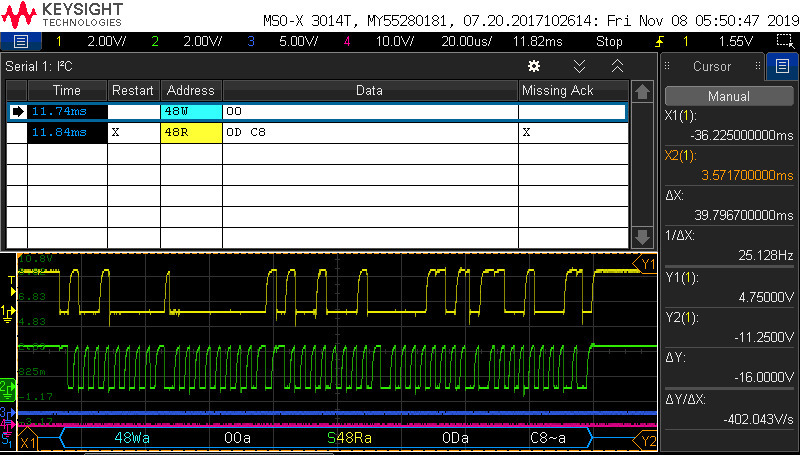
\includegraphics[width=\linewidth]{images/i2c/i2c_lister.jpg}
      \caption{}
      \label{fig:i2c_lister}
    \end{subfigure}
    \caption{
      I\textsuperscript{2}C Bus (a) Without Lister Menu and (b) With Lister Menu
    }
    % \caption{I2C Bus With (b) and Without Lister Menu(a)}
    \label{fig:i2c_decode}
  \end{figure}

  \section{Microcontroller Execution Time Measurement}

  \subsection{Required Equipment}

  To be able to measure execution time on a microcontroller, the microcontroller
  needs to be able to signal when an execution begins and when it ends. The
  easiest way for a microcontroller to signal when something begins and ends is
  to change the state of a general purpose output. Using an oscilloscope, the
  duration between changes in output can easily be measured.  Fortunately, this
  is one of the more accurate methods to measure execution time.

  \subsection{Setup}

  To make the measurement, an output pin will need to be set high immediately
  before entering the code in question. The pin should then be set to low again
  after exiting the block of code. Once the microcontroller is ready, the
  oscilloscope requires a few preparations to perform this measurement.

  Only one oscilloscope probe is needed to perform this measurement. The scope
  needs to be set to trigger on the channel that the probe is connected to. In
  the example, the probe is connected to channel one, so channel one is selected
  in the trigger menu shown in figure~\ref{fig:exectime_trigger}. With the
  channel configured to trigger on a rising edge, the oscilloscope should be set
  to single mode so that a single event is captured at a time. Now the
  oscilloscope is ready to make the measurement.

  % TODO add trigger menu
  \begin{figure}[h]
    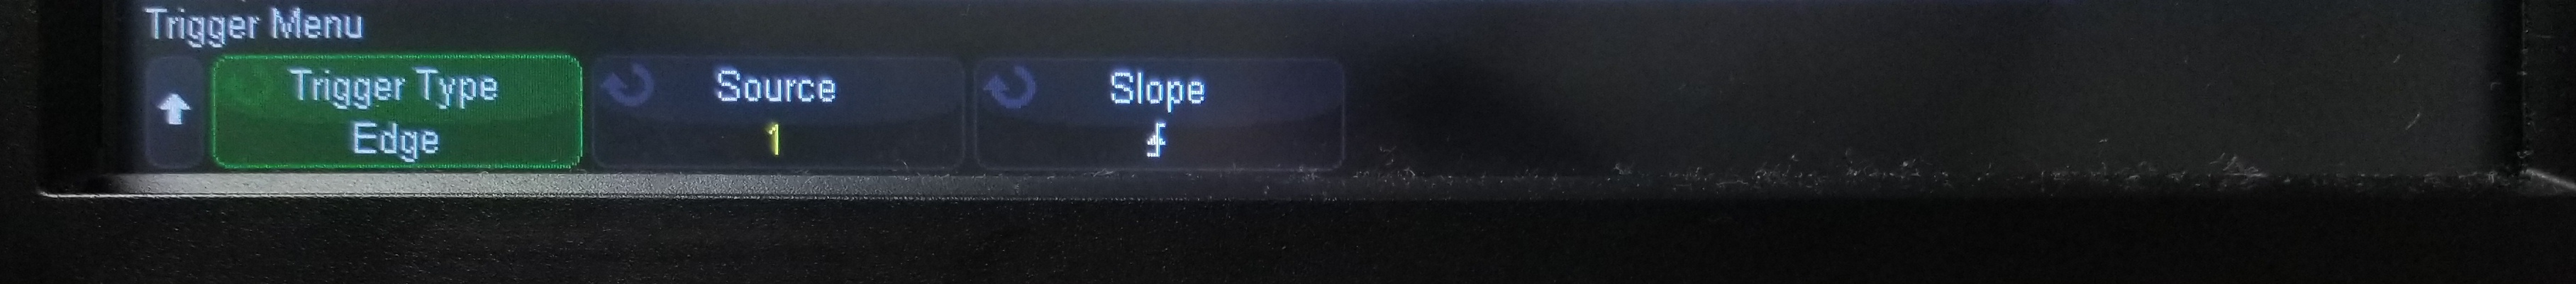
\includegraphics[width=\textwidth]{images/exec_time/trigger_menu.jpg}
    \caption{Trigger settings menu. Channel 1 is selected as the trigger source
      and the oscilloscope is set to trigger on the rising edge.}
    \label{fig:exectime_trigger}
  \end{figure}

  Start the microcontroller and wait for the oscilloscope to display a single
  rise and fall on the screen. If the display only show a rise and no fall, the
  time scale will need to be extended and the measurement recaptured until both
  beginning and end times can be seen. With both rise and fall visible on the
  display, the cursor functionality on the oscilloscope can be used to estimate
  the duration.

  \subsection{Results}

  Our example execution time was simply a sleep function to check its accuracy.
  The delay was set to last for 5 milliseconds,
  Figure~\ref{fig:exectime_measure} shows that our sleep function ran just over
  the intended duration. The cursors on the oscilloscope are set one on the
  rising edge of the signal and one of the falling edge. The oscilloscope now
  calculates the difference between these cursors corresponding times and shows
  the duration on the right as can be seen in Figure~\ref{fig:exectime_measure}.

  \begin{figure}[h]
    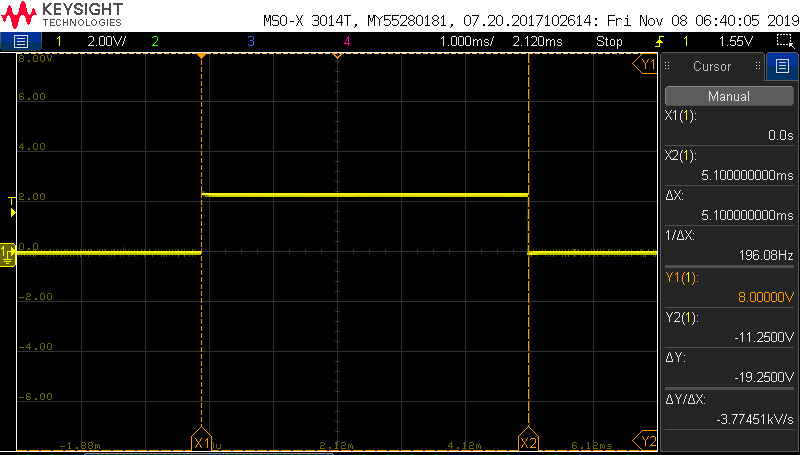
\includegraphics[width=\textwidth]{images/exec_time/exec_time.jpg}
    \caption{Execution Time Measurement}
    \label{fig:exectime_measure}
  \end{figure}

  \section{External Debugger Setup}

  \subsection{Required Equipment}

  \begin{wrapfigure}{l}{30ex}
    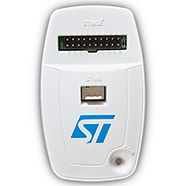
\includegraphics[width=30ex]{images/programming/stlinkv2.jpg}
    \caption{ST-LINK V2 \\ Programmer}
  \end{wrapfigure}

  To debug a microcontroller externally, a debugger or programmer will be
  required. There are many different microcontrollers and programmers available,
  but this document will only discuss the use of the ST-LINK to program and
  debug STM32 microcontrollers using SWD or Serial Wire Debugging. More
  specifically, an NUCLEO-F401RE development board will be used to demonstrate
  the procedure, but the steps should remain similar for all STM32
  microcontrollers when programmed with the ST-LINK programmer.

  \subsection{Setup}

  The ST-LINK programmer only requires four connections, VDD, GND, SWDIO, and
  SWCLK. While these are sufficient, connecting nRST between programmer and
  microcontroller is often beneficial and highly recommended.
  Figure~\ref{fig:stlink_pinout} shows the connections on the ST-LINK V2
  programmer needed to program an STM32 microcontroller.

  \begin{figure}[h]
    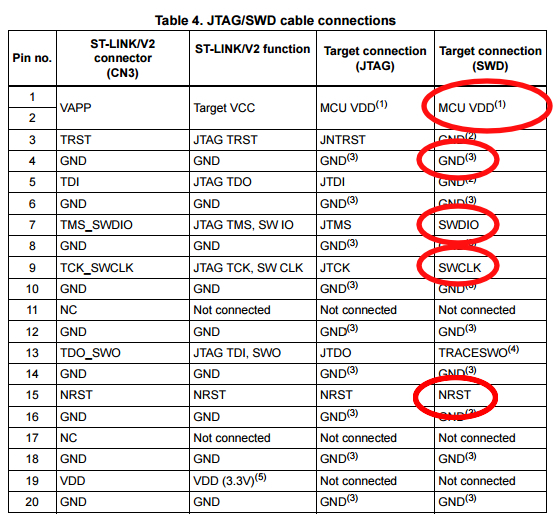
\includegraphics[width=0.55\textwidth]{images/programming/stlink-pinout-circled.jpg}
    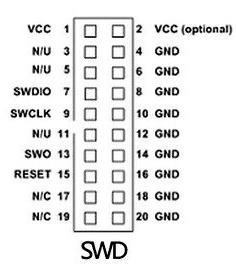
\includegraphics[width=0.45\textwidth]{images/programming/swd_connector.jpg}
    \caption{ST-LINK V2 connections and pin layout}
    \label{fig:stlink_pinout}
  \end{figure}

  The associated pins on the microcontroller should be listed in the datasheet.
  Figure~\ref{fig:nucleo_swd_connections} shows the connections for the
  NUCLEO-F401RE development board. It is important to note that even with VCC
  connected between board and programmer, the microcontroller still requires
  external power.  As with most development boards the NUCLEO has an ST-LINK
  included on the board. The connections for this embedded ST-LINK are also
  indicated in Figure~\ref{fig:nucleo_swd_connections}. If a development board
  is available, a dedicated ST-LINK programmer is not necessary to program an
  embedded STM32 Microcontroller, instead a development board can serve this
  purpose.

  \begin{figure}[ht]
    \centering
    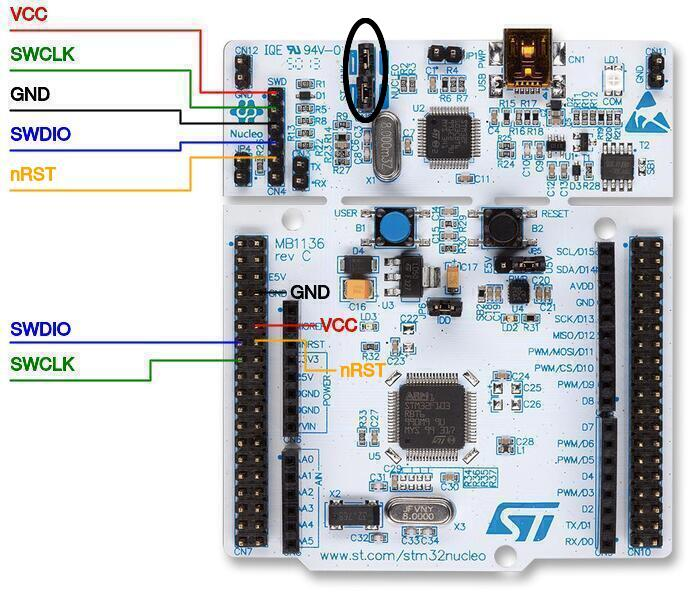
\includegraphics[width=.65\textwidth]{images/programming/stm32_nucleo_f401re_connections.jpg}
    \caption{SWD Programming connections on STM32F401RE Development Board}
    \label{fig:nucleo_swd_connections}
  \end{figure}

  \begin{figure}[ht]
    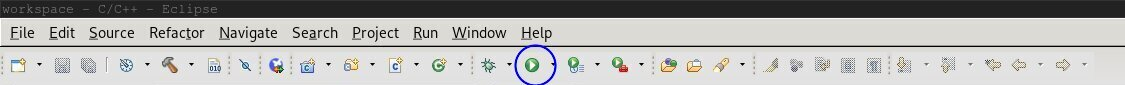
\includegraphics[width=\textwidth]{images/programming/syswb_flash.jpg}
    \caption{Flashing a program to the microcontroller with System Workbench}
  \end{figure}

  The black circle in Figure~\ref{fig:nucleo_swd_connections} indicates the
  jumpers that need to be removed to use an embedded ST-LINK to flash an
  externam microcontroller. These jumpers connect the embedded ST-LINK to the
  microcontroller on the development board, but when they are removed, the
  headers can be used to connect to an external microcontroller.

  With all required connections made, the regular method of flashing a program
  to the microcontroller can be used. In this example, System Workbench is used
  to program the microcontrollers, and if everything is connected properly, it
  should proceed exactly as before. If anything is connected improperly, System
  Workbench will produce an error message, usually about a wrong device being
  connected, or no device being connected to the ST-LINK.

  \clearpage

  \subsection{Results}

  When everything is connected properly, System Workbench or whatever software
  used to program the microcontroller should continue to work exactly as it did
  while connected directly to the development board for the microcontroller
  because, in essence, the communication between computer and microcontroller is
  still the same through either ST-LINK that is being used.

\end{document}
